Wearable robotic devices are intended as a means to augment human economy, strength, and endurance. Over the past decade, a number of devices have been developed for reducing the metabolic cost of walking for able-bodied individuals \citep{Malcolm2013, Mooney2016, Caputo2014,  Panizzolo2016}. With tethered and portable hardware platforms having advanced considerably \citep{Malcolm2013, Lee2018, Panizzolo2015}, it is now possible to accurately control settings such as the timing and magnitude of the delivered torque \citep{Malcolm2013, Collins2015, Ding2017, Kim2015, Kim2017inv, Lee2016}. Increased attention has been directed towards how control strategy and control parameters influence overall system performance \citep{Caputo2014, Kim2015, Kim2017inv, Quinlivan2017}. Traditionally, control parameters have been tuned manually by researchers with expert knowledge on both the device and biomechanics of human walking or through exploring the parameter space in a systematic sweep \citep{Caputo2015, Quinlivan2017}. However, despite these efforts, several studies have shown significant inter-subject variability in the observed metabolic benefit for a fixed parameter setting~\citep{Quesada2016}. Being able to automatically recover the optimal parameter setting on an individual basis is therefore a fundamental component in designing effective wearable robotic devices.

Recently, several groups have explored different formulations of \emph{human-in-the-loop} (HIL) optimization that offer the possibility to avoid conventional exhaustive search~\citep{Koller2016, Zhang2017, Ding2018, Kim2017}. These studies use instantaneous energetic cost~\citep{Selinger2014}, an estimation of steady-state metabolic cost, as an objective measurement for automatically optimizing parameter settings~\citep{Koller2016, Felt2015, Zhang2017, Ding2018}. Previous research has applied this HIL optimization approach to find optimal onset actuation timing of a bilateral pneumatic ankle exoskeleton by automatically adjusting a single control parameter~\citep{Koller2016}. A recent study with an ankle exoskeleton~\citep{Zhang2017} and hip exosuit~\citep{Ding2018} showed the potential to achieve larger metabolic benefits by simultaneously optimizing multiple parameters using \emph{Bayesian optimization}.

\section*{Motivation}
Bayesian optimization is a sequential optimization strategy that has been used in a variety of applications from hyperparameter tuning for machine learning algorithms~\citep{NIPS2012_4522,pmlr-v22-mahendran12} to portfolio allocation \citep{1009.5419} and experimental design \citep{Brochu2009}. As it is a general framework to optimize noisy black box functions, many variations have been introduced to account for different use cases. In particular, an area of interest has been in tackling the noisiness of data samples \citep{rue2009,1603.02038,1410.7172} and the myopia of the algorithm \citep{NIPS2016_6188,1510.06299}. 

The algorithm is typically framed in the context of an iteration budget, abstracting away the actual data sampling process. However, in the HIL problem there is a limited time constraint rather than an iteration constraint, and data acquisition exhibits a direct tradeoff between noisiness and elapsed time. In previous studies, a fixed observation window was used for every parameter evaluation, effectively reducing the time constraint to an iteration constraint. Unfortunately, this means spending valuable time measuring parameter settings that are unlikely to improve upon the best value observed so far.

\begin{figure}
\centering
\tikzstyle{startstop} = [rectangle, rounded corners, minimum width=3cm, minimum height=1cm,text centered, text width=3cm, draw=black, fill=red!30]
\tikzstyle{process} = [rectangle, minimum width=3cm, minimum height=1cm, text centered, text width=2.5cm, draw=black, fill=orange!30]
\tikzstyle{decision} = [rectangle, minimum width=3cm, minimum height=1cm, text centered, text width=2.5cm, draw=black, fill=green!30]
\tikzstyle{arrow} = [thick,->,>=stealth]
    
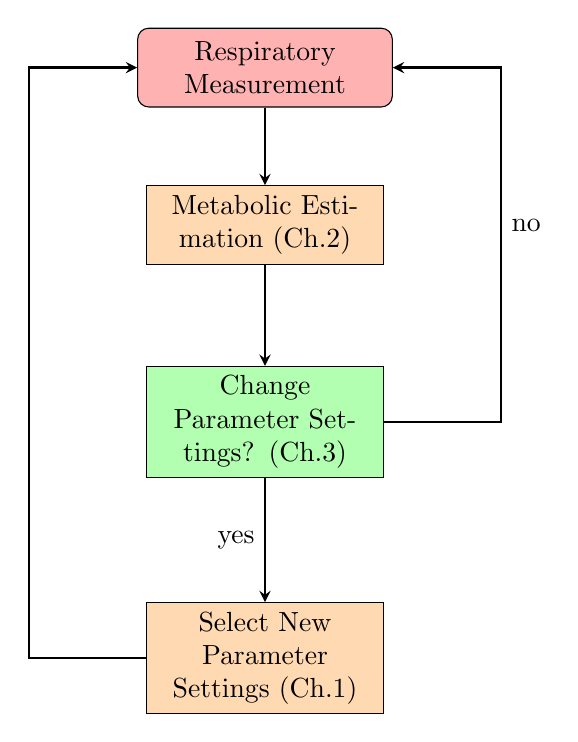
\begin{tikzpicture}[node distance=2cm]

\node (measurement) [startstop] {Respiratory Measurement};
\node (estimator) [process, below of=measurement] {Metabolic Estimation (Ch.2)};
\node (stopping) [decision, below of=estimator, yshift=-0.5cm] {Change Parameter Settings? (Ch.3)};
\node (bayesopt) [process, below of=stopping, yshift=-1cm] {Select New Parameter Settings (Ch.1)};

\draw [arrow] (measurement) -- (estimator);
\draw [arrow] (estimator) -- (stopping);
\draw [arrow] (stopping) --++ (3cm,0cm) |- node[anchor=west, yshift=-2cm] {no} (measurement);
\draw [arrow] (stopping) -- node[anchor=east] {yes} (bayesopt);
\draw [arrow] (bayesopt) --++ (-3cm,0cm) |- (measurement);


\end{tikzpicture}
\caption{Flow diagram of optimization problem}
\end{figure}

\section*{Summary of contributions}
The main contribution of this work is to introduce a stopping problem within a given evaluation of Bayesian optimization. Rather than having a fixed observation window, a stopping rule is determined after every respiratory measurement to maximize the time spent evaluating promising parameter settings. To determine the optimal stopping time, a metabolic cost estimator\footnote{Primary development by Myunghee Kim} is also developed to provide a probability distribution of the instantaneous energetic cost after every measurement. Depending on the paramterization of the estimator, two  formulations of the stopping problem are introduced and evaluated under different circumstances.

\section*{Outline}
Chapter \ref{ch:1} gives background information on Bayesian optimization and Gaussian processes. Chapter \ref{ch:2} presents the metabolic estimator and its robustness under various levels of noise. Initial experimental data is provided and future work on the estimator is discussed. Chapter \ref{ch:3} introduces two algorithms for determining the optimal stopping point within an iteration of Bayesian Optimization. Simulations of various optimization functions are provided using the two algorithms under different scenarios. Chapter \ref{ch:4} provides results from an experimental protocol using one of the algorithms. Finally, we conclude this thesis with a discussion of future work.